% Choose one to switch between slides and handout
\documentclass[]{beamer}
%\documentclass[handout]{beamer}

% Video Meta Data
\title{Bitcoin, Blockchain and Cryptoassets}
\subtitle{Peer-to-Peer Networks}
\author{Prof. Dr. Fabian Schär}
\institute{University of Basel}

% Config File
% Packages
\usepackage[utf8]{inputenc}
\usepackage{hyperref}
\usepackage{gitinfo2}
\usepackage{tikz}
\usepackage{amsmath}
\usepackage{bibentry}
\usepackage{xcolor}
\usepackage{colortbl} % Add colour to LaTeX tables
\usepackage{caption}
\usepackage[export]{adjustbox}
\usepackage{pgfplots} \pgfplotsset{compat = 1.17}

% Color Options
\definecolor{highlight}{rgb}{0.65,0.84,0.82}
\definecolor{focus}{rgb}{0.72, 0, 0}

% Beamer Template Options
\beamertemplatenavigationsymbolsempty
\setbeamertemplate{footline}[frame number]
\setbeamercolor{structure}{fg=black}
\setbeamercolor{footline}{fg=black}
\setbeamercolor{title}{fg=black}
\setbeamercolor{frametitle}{fg=black}
\setbeamercolor{item}{fg=black}
\setbeamercolor{}{fg=black}
\setbeamercolor{bibliography item}{fg=black}
\setbeamercolor*{bibliography entry title}{fg=black}
\setbeamertemplate{items}[square]
\setbeamertemplate{enumerate items}[default]
\captionsetup[figure]{labelfont={color=black},font={color=black}}
\captionsetup[table]{labelfont={color=black},font={color=black}}

\setbeamertemplate{bibliography item}{\insertbiblabel}

% Link Icon Command
\newcommand{\link}{%
    \tikz[x=1.2ex, y=1.2ex, baseline=-0.05ex]{%
        \begin{scope}[x=1ex, y=1ex]
            \clip (-0.1,-0.1)
                --++ (-0, 1.2)
                --++ (0.6, 0)
                --++ (0, -0.6)
                --++ (0.6, 0)
                --++ (0, -1);
            \path[draw,
                line width = 0.5,
                rounded corners=0.5]
                (0,0) rectangle (1,1);
        \end{scope}
        \path[draw, line width = 0.5] (0.5, 0.5)
            -- (1, 1);
        \path[draw, line width = 0.5] (0.6, 1)
            -- (1, 1) -- (1, 0.6);
        }
    }

% Read Git Data from Github Actions Workflow
% Defaults to gitinfo2 for local builds
\IfFileExists{gitInfo.txt}
	{\input{gitInfo.txt}}
	{
		\newcommand{\gitRelease}{(Local Release)}
		\newcommand{\gitSHA}{\gitHash}
		\newcommand{\gitDate}{\gitAuthorIsoDate}
	}

% Custom Titlepage
\defbeamertemplate*{title page}{customized}[1][]
{
  \vspace{-0cm}\hfill
\includegraphics[width=2.5cm]{../config/logo_cif}
  
\includegraphics[width=1.9cm]{../config/seal_wwz}
  \\ \vspace{2em}
  \usebeamerfont{title}\textbf{\inserttitle}\par
  \usebeamerfont{title}\usebeamercolor[fg]{title}\insertsubtitle\par  \vspace{1.5em}
  \small\usebeamerfont{author}\insertauthor\par
  \usebeamerfont{author}\insertinstitute\par \vspace{2em}
  \usebeamercolor[fg]{titlegraphic}\inserttitlegraphic
    \tiny \noindent \texttt{Release Ver.: \gitRelease}\\ 
    \texttt{Version Hash: \gitSHA}\\
    \texttt{Version Date: \gitDate}\\ \vspace{1em}
  \link \href{https://github.com/cifunibas/Bitcoin-Blockchain-Cryptoassets/blob/main/slides/intro.pdf}
  {Get most recent version}\\
  \link \href{https://github.com/cifunibas/Bitcoin-Blockchain-Cryptoassets/blob/main/slides/intro.pdf}
  {Watch video lecture}\\ \vspace{1em}
  License: \texttt{Creative Commons Attribution-NonCommercial-ShareAlike 4.0 International}\\\vspace{2em}
  
\includegraphics[width = 1.2cm]{../config/license}
}

% tikzlibraries
\usetikzlibrary{decorations.pathreplacing}
\usetikzlibrary{decorations.markings}
\usetikzlibrary{positioning}

%caption font
\captionsetup{font=footnotesize}


%%%%%%%%%%%%%%%%%%%%%%%%%%%%%%%%%%%%%%%%%%%%%%
%%%%%%%%%%%%%%%%%%%%%%%%%%%%%%%%%%%%%%%%%%%%%%

\begin{document}

\thispagestyle{empty}
\begin{frame}[noframenumbering]
	\titlepage
\end{frame}

%%%
\begin{frame}{The Origin of Peer-to-Peer Networks}
	Peer-to-peer (p2p) networks were popularized by file sharing systems in the early 2000s.
	\begin{columns}
		\begin{column}{0.5\textwidth}
			\begin{figure}
				\begin{center}
					
\includegraphics[height = 0.25\textheight]{../assets/images/napster}
				\end{center}
			\end{figure}
		\end{column}
		\begin{column}{0.5\textwidth}
			\begin{figure}
				\begin{center}
					
\includegraphics[height = 0.16\textheight]{../assets/images/limewire}
				\end{center}
			\end{figure}
		\end{column}
	\end{columns}
	\begin{columns}
		\begin{column}{0.5\textwidth}
			\begin{center}
				Napster
			\end{center}
		\end{column}
		\begin{column}{0.5\textwidth}
			\begin{center}
				LimeWire
			\end{center}
		\end{column}
	\end{columns}
	\vspace{1.8em}
	\uncover<2->{They allow network participants to directly interact with eachother, without the need for servers or stable hosts.}
\end{frame}
%%%

%%%
\begin{frame}{Peer-to-Peer vs. Centralized Networks}
	\vspace{1em}
	In a peer-to-peer network, each participant...
	\vspace{0.5em}
%	\begin{footnotesize}
		\begin{itemize}
			\item<2-> Can connect to any number of other participants
			\item<3-> Has equal privileges (no administration)
			\item<4-> Is consumer and provider of resources (client and server)
		\end{itemize}
%	\end{footnotesize}
	\begin{columns}[T]
		\begin{column}{0.5\textwidth}
			\vspace{2.5em}
			\begin{tikzpicture}[scale=0.7, every node/.style={scale=0.7}]
				
% Title
%\node[above] at (2,4.3) {Peer-to-Peer};


% Network
\node (agenta) at (1,2.8) {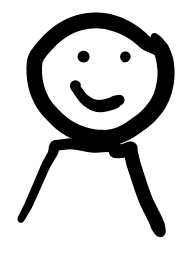
\includegraphics[width = 0.6 cm]{../assets/images/agents/avatar_rand3.png}};
\node (agentb) at (0.5,1) {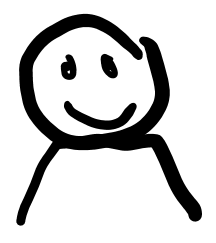
\includegraphics[width = 0.6 cm]{../assets/images/agents/avatar_rand4.png}};
\node (agentc) at (3,2.1) {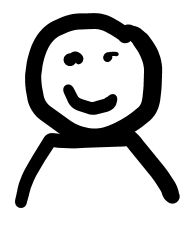
\includegraphics[width = 0.6 cm]{../assets/images/agents/avatar_rand5.png}};
\node (agentd) at (2.8,0) {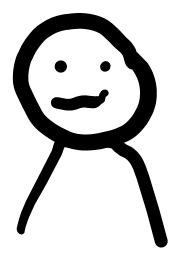
\includegraphics[width = 0.6 cm]{../assets/images/agents/avatar_rand1.png}};
\node (agente) at (5,4.3) {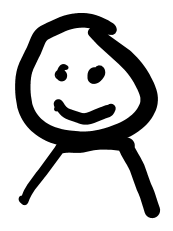
\includegraphics[width = 0.6 cm]{../assets/images/agents/avatar_rand2.png}};	
\node (agentf) at (5.1,1.1) {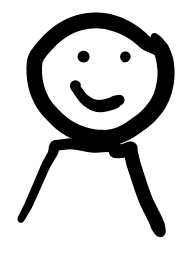
\includegraphics[width = 0.6 cm]{../assets/images/agents/avatar_rand3.png}};
\node (agentg) at (7.5,3.8) {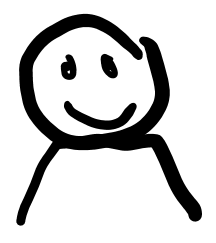
\includegraphics[width = 0.6 cm]{../assets/images/agents/avatar_rand4.png}};
\node (agenth) at (6.7,0.4) {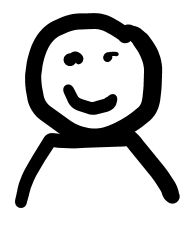
\includegraphics[width = 0.6 cm]{../assets/images/agents/avatar_rand5.png}};

% Network flow
\draw[<->, thick, dashed]	(agenta.south) -- (agentb.north);
\draw[<->, thick, dashed] 	(agenta.east) -- (agente.west);
\draw[<->, thick, dashed]	(agenta.south east) -- (agentc.west);
\draw[<->, thick, dashed]	(agente.south west) -- (agentc.north east);
\draw[<->, thick, dashed]	(agente.south) -- (agentf.north);
\draw[<->, thick, dashed]	(agente.east) -- (agentg.west);
\draw[<->, thick, dashed]	(agentc.south west) -- (agentb.east);
\draw[<->, thick, dashed]	(agentc.south) -- (agentd.north);
\draw[<->, thick, dashed]	(agentc.south east) --  (agentf.west);
\draw[<->, thick, dashed]	(agentg.south west) -- (agentf.north east);
\draw[<->, thick, dashed]	(agentg.south) -- (agenth.north);
\draw[<->, thick, dashed]	(agentb.south east) -- (agentd.west);
\draw[<->, thick, dashed]	(agentf.south west) -- (agentd.east);
\draw[<->, thick, dashed]	(agentf.south east) -- (agenth.west);
\draw[<->, thick, dashed]	(agenth.south west) -- (agentd.east);

			\end{tikzpicture}
		\end{column}
		\begin{column}{0.5\textwidth}
			\begin{tikzpicture}[scale=0.7, every node/.style={scale=0.7}]
				
% Title
\node[above] at (2.5,5.5) {Centralized};


% Network
\node (server) at (4.5,2.8) {
\includegraphics[width = 0.5 cm]{../assets/images/agents/intermediary.png}};
\node (agenta) at (1,4.7) {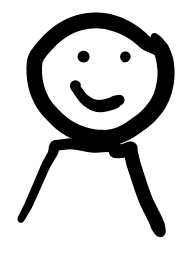
\includegraphics[width = 0.6 cm]{../assets/images/agents/avatar_rand3.png}};
\node (agentb) at (0.5,2) {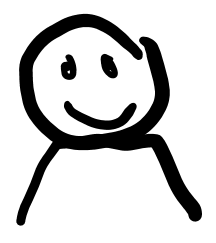
\includegraphics[width = 0.6 cm]{../assets/images/agents/avatar_rand4.png}};
\node (agentc) at (2.8,0) {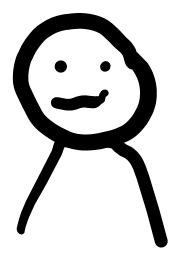
\includegraphics[width = 0.6 cm]{../assets/images/agents/avatar_rand1.png}};
\node (agentd) at (5,5.7) {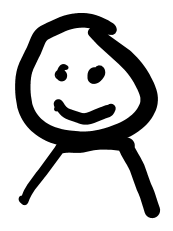
\includegraphics[width = 0.6 cm]{../assets/images/agents/avatar_rand2.png}};	
\node (agente) at (7.5,3.8) {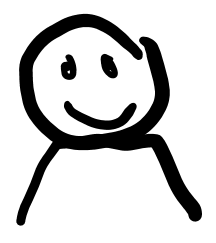
\includegraphics[width = 0.6 cm]{../assets/images/agents/avatar_rand4.png}};
\node (agentf) at (6.7,0.2) {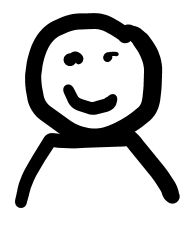
\includegraphics[width = 0.6 cm]{../assets/images/agents/avatar_rand5.png}};

% Network flow
\draw[<->, thick, dashed]	(agenta.east) -- (server.north west);
\draw[<->, thick, dashed] 	(agentb.east) -- (server.west);
\draw[<->, thick, dashed]	(agentc.north east) -- (server.south west);
\draw[<->, thick, dashed]	(agentd.south) -- (server.north);
\draw[<->, thick, dashed]	(agente.west) -- (server.east);
\draw[<->, thick, dashed]	(agentf.north west) -- (server.south east);


			\end{tikzpicture}
		\end{column}
	\end{columns}
\end{frame}
%%%


%%%
\begin{frame}{Node Software}
	\centering
	\begin{tikzpicture}[scale=0.7, every node/.style={scale=1}]
		
\begin{tikzpicture}[scale = 0.67]
	
	\definecolor {dgray}{rgb}{122,122,122}
	\definecolor {lgray}{rgb}{194,194,194}
	
	% Title
%	\node[draw, align=center] at (2.2,4.5) {Peer-to-Peer};
%	

	
	% Agents
	\node (agenta) at (1,0) {
\includegraphics[height = 2 cm]{../assets/images/agents/avatar_discover}};
	\uncover<-1>{\node (agentc) at (10,0) {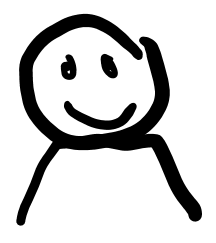
\includegraphics[height = 2 cm, decodearray={0.6 0 0.6 0 0.6 0}] {../assets/images/agents/avatar_rand4}};} % grayed out agent for first slide
	\uncover<2->{\node (agentb) at (10,0) {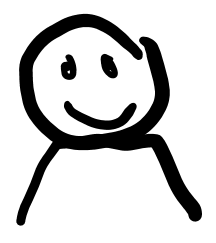
\includegraphics[height = 2 cm] {../assets/images/agents/avatar_rand4}};}
	
	\node[above] at (agenta.north) {Discover};
	
	% Actions
	\uncover<2->{\draw[<->, thick, dashed]	(agenta.east) -- node [above] {Connect} (agentb.west);}
	\uncover<3->{\draw[->, thick, dashed]	(agenta.north east) -- node [above] {Share} (agentb.north west);}
	\uncover<4->{\draw[<-, thick, dashed]	(agenta.south east) -- node [above] {Access} (agentb.south west);}
	
\end{tikzpicture}

	\end{tikzpicture}
%	\vspace{.5 cm}
%	Node software functionality:
%	\begin{enumerate}
%		\item Discover other nodes
%		\item<2-> Connect to discovered nodes
%		\item<3-> Share resources with peers
%		\item<4-> Access resources from peers
%	\end{enumerate}
\end{frame}
%%%

%%%
\begin{frame}{Network Specification}
	\begin{center}
		\begin{tikzpicture}[scale=0.7, every node/.style={scale=1}]
			
\begin{tikzpicture}[scale = 0.67]
	
	% Agents
	\node (agenta) at (1,0) {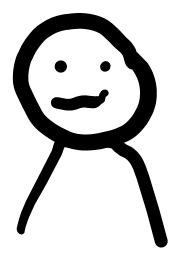
\includegraphics[height = 2 cm]{../assets/images/agents/avatar_rand1}};
	\node (agentb) at (10,0) {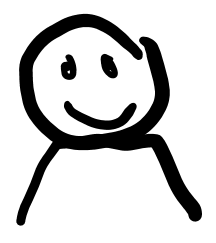
\includegraphics[height = 2 cm] {../assets/images/agents/avatar_rand4}};
	
	% Text
	\node[below] (clienta) at (agenta.south) {Software A};
	\node[below] (clientb) at (agentb.south) {Software B};
	
	% Actions
	\draw[<->, thick, dashed]	(agenta.east) -- node [above] {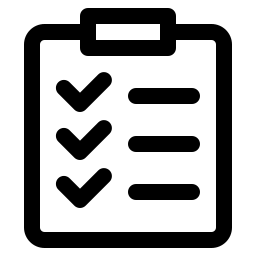
\includegraphics[height = 1.5 cm]{../assets/images/checklist}} (agentb.west);

	
\end{tikzpicture}

		\end{tikzpicture}
	\end{center}
	\vspace{.5 cm}
	
	Node communication is defined by the \color{focus}protocol specifications\color{black}.
	\begin{itemize}
		\item<2-> Nodes can run different software implementations
		\item<3-> Allows specialization of nodes
		\item<3-> \color{focus}Further decentralizes \color{black}the system
	\end{itemize}
\end{frame}
%%%

%%%
\begin{frame}{Peer Discovery}
	\begin{center}
		\begin{tikzpicture}[scale=1, every node/.style={scale=1}]
			
\definecolor{Redish}{rgb}{0.8,0.5,0.5}

% Network
\node (agentc) at (3,2.1) {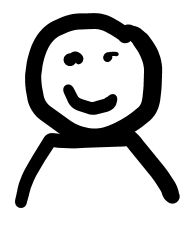
\includegraphics[width = 0.6 cm]{../assets/images/agents/avatar_rand5}};

\node (agenta) at (1,2.8) {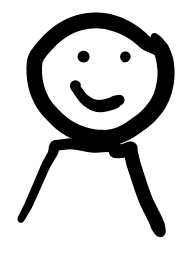
\includegraphics[width = 0.6 cm, decodearray={0.8 0 0.8 0 0.8 0}]{../assets/images/agents/avatar_rand3.png}};
\node (agentb) at (0,1) {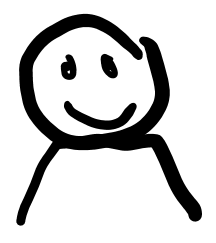
\includegraphics[width = 0.6 cm, decodearray={0.8 0 0.8 0 0.8 0}]{../assets/images/agents/avatar_rand4}};
\node (agentd) at (2.8,0) {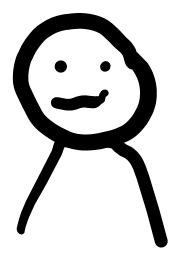
\includegraphics[width = 0.6 cm, decodearray={0.8 0 0.8 0 0.8 0}]{../assets/images/agents/avatar_rand1}};
\node (agente) at (5,4.3) {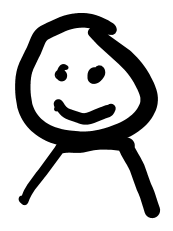
\includegraphics[width = 0.6 cm, decodearray={0.8 0 0.8 0 0.8 0}]{../assets/images/agents/avatar_rand2}};	
\node (agentf) at (5.1,1.1) {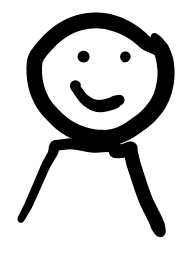
\includegraphics[width = 0.6 cm, decodearray={0.8 0 0.8 0 0.8 0}]{../assets/images/agents/avatar_rand3}};
\node (agentg) at (8,3.4) {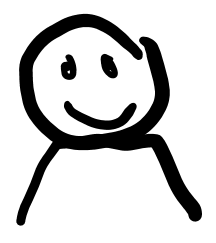
\includegraphics[width = 0.6 cm, decodearray={0.8 0 0.8 0 0.8 0}]{../assets/images/agents/avatar_rand4}};
\node (agenth) at (6.7,0.4) {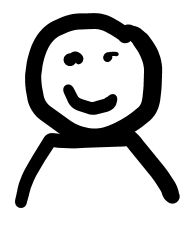
\includegraphics[width = 0.6 cm, decodearray={0.8 0 0.8 0 0.8 0}]{../assets/images/agents/avatar_rand5}};

% Network flow
\color{lightgray}
\draw[<->, thick, dashed]	(agenta.south east) -- (agentd.north west);
\draw[<->, thick, dashed]	(agenta.south west) -- (agentb.north);
\draw[<->, thick, dashed] 	(agenta.north east) -- (agente.west);
\draw[<->, thick, dashed]	(agente.south) -- (agentf.north);
\draw[<->, thick, dashed]	(agente.east) -- (agentg.north west);
\draw[<->, thick, dashed]	(agentg.south west) -- (agentf.north east);
\draw[<->, thick, dashed]	(agentg.south) -- (agenth.north);
\draw[<->, thick, dashed]	(agentb.south east) -- (agentd.west);
\draw[<->, thick, dashed]	(agentf.south west) -- (agentd.east);
\draw[<->, thick, dashed]	(agentf.south east) -- (agenth.west);
\draw[<->, thick, dashed]	(agenth.south west) -- (agentd.east);
\color{black}

\uncover<2->{
	\node (agente2) at (agente) {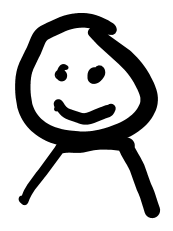
\includegraphics[width = 0.6 cm]{../assets/images/agents/avatar_rand2}};	
	
	\draw[<->, thick, dashed] 	(agentc.north east) -- (agente.south west);
}

\uncover<3-3>{
	\node (agenta2) at (agenta) {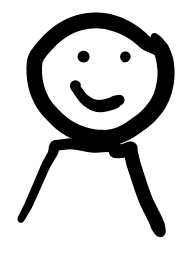
\includegraphics[width = 0.6 cm, decodearray={0.8 0 0.5 0 0.5 0}]{../assets/images/agents/avatar_rand3}};
	\node (agentf2) at (agentf) {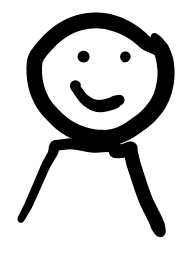
\includegraphics[width = 0.6 cm, decodearray={0.8 0 0.5 0 0.5 0}]{../assets/images/agents/avatar_rand3}};	
	\node (agentg2) at (agentg) {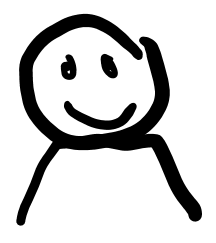
\includegraphics[width = 0.6 cm, decodearray={0.8 0 0.5 0 0.5 0}]{../assets/images/agents/avatar_rand4}};		
	
	\color{Redish}
	\draw[<->, thick, dashed] 	(agenta.north east) -- (agente.west);
	\draw[<->, thick, dashed]	(agente.south) -- (agentf.north);
	\draw[<->, thick, dashed]	(agente.east) -- (agentg.north west);
	\color{black}
}

\uncover<4->{
	\node (agenta2) at (agenta) {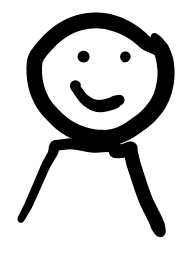
\includegraphics[width = 0.6 cm]{../assets/images/agents/avatar_rand3}};
	\node (agentf2) at (agentf) {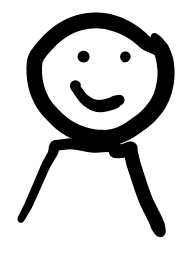
\includegraphics[width = 0.6 cm]{../assets/images/agents/avatar_rand3}};	
	
	\draw[<->, thick, dashed]	(agentc.west) -- (agenta.east);
	\draw[<->, thick, dashed]	(agentc.south east) -- (agentf.west);
}

\uncover<5->{
	\node (agentg2) at (agentg) {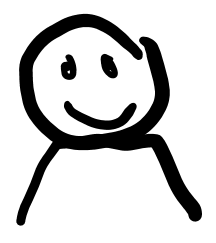
\includegraphics[width = 0.6 cm]{../assets/images/agents/avatar_rand4}};	
	\node (agentd2) at (agentd) {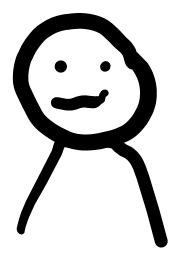
\includegraphics[width = 0.6 cm]{../assets/images/agents/avatar_rand1}};	
	
	\draw[<->, thick, dashed]	(agentg.west) -- (agentc.east);
	\draw[<->, thick, dashed]	(agentc.south) -- (agentd.north);
	
}


		\end{tikzpicture}
	\end{center}
	%\vspace{0.5 cm}
	\uncover<2->{Basic peer discovery:}
	\begin{enumerate}
		\item<2-> Connect to a known peer
		\item<3-> Ask this peer for a list of their connections
		\item<4-> Connect to a random set of peers from this list
		\item<5-> Repeat steps 2 and 3 until enough connections are established
	\end{enumerate}
\end{frame}
%%%

%%%
\begin{frame}{Advantages of P2P Networks}
	A peer-to-peer architecture offers key advantages:
	\vspace{0.3 cm}
	\begin{itemize}
		\item No central point of failure
		\begin{itemize}
			\item No single node is critical for a functioning network
			\item No bandwidth bottlenecks
		\end{itemize}
		\vspace{0.3 cm}
		\item<2-> No central point for an attack
			\begin{itemize}
				\item No node has special privileges or powers
				\item Very difficult to overload the network via DoS attacks
			\end{itemize}	
		\vspace{0.3 cm}
		\item<3-> Every peer supplies hardware
		\vspace{0.3 cm}
		\item<4-> Difficult to regulate or stop
	\end{itemize}
	
\end{frame}
%%%

%%%
\begin{frame}{Problems of P2P Networks}
	Trade-offs have to be made, especially regarding security:
	\vspace{0.3 cm}
	\begin{itemize}
		\item A node can share malicious or irrelevant resources
		\vspace{0.3 cm}
		\item<2-> Difficult to regulate illicit activity
		\vspace{0.3 cm}
		\item<3-> Limited by the nodes with the weakest hardware
	\end{itemize}
	
\end{frame}
%%%


\begin{frame}%[allowframebreaks]
\frametitle{Further Reading}
		\textbf{Cryptocurrency Networks: A New P2P Paradigm}, \\
		Delgado-Segura et al., 2018, Mobile Information Systems, \\
		\link \url{https://doi.org/10.1155/2018/2159082}
\end{frame}

\end{document}